%************************************************
\chapter{Prior Work}\label{ch:prior-work}
%**************************************

\todotext{textbox}

Prior to 2017, when the first work presented in this thesis was
published, there was only limited literature on EEG decoding with deep
learning. In this chapter, I outline what decoding problems, input
representations, network architectures, hyperparameter choices and
visualizations were evaluated in prior work. This is based on the
literature research that we presented in
\citet{schirrmeisterdeephbm2017}.

\section{Decoding Problems and
Baselines}\label{decoding-problems-and-baselines}


% \end{longtable}


\begin{table}[th]
    \myfloatalign
    \begin{tabularx}{\textwidth}{p{0.5\textwidth}p{0.2\textwidth}p{0.2\textwidth}} \toprule
        \tableheadlinewithwidth{0.5\textwidth}{Decoding problem} & \tableheadlinewithwidth{0.2\textwidth}{Number of studies}
        & \tableheadlinewithwidth{0.2\textwidth}{Published baseline} \\ 
        \midrule
    Imagined or Executed Movement & 6 & 2 \\
    Oddball/P300 & 5 & 1 \\
    Epilepsy-related & 4 & 2 \\
    Music Rhythm & 2 & 0 \\
    Memory Performance/Cognitive Load & 2 & 0 \\
    Driver Performance & 1 & 0 \\
        \bottomrule
    \end{tabularx}
    \caption[Decoding problems in deep-learning EEG decoding studies prior to our work.]{\textbf{Decoding problems in deep-learning EEG decoding studies prior to our work.} Studies with published baseline compared their decoding results to an external baseline result published by other authors.}  \label{prior-work-tasks-table}
\end{table}



    The most widely studied decoding problems were movement-related decoding
problems such as decoding which body part (hand, feet etc.) a person is
moving or imagining to move (see
\Cref{prior-work-tasks-table}). From the 19 studies we
identified at the time, only 5 compared their decoding results to an
external published baseline result, limiting the insights about
deep-learning EEG decoding performance. We therefore decided to compare
deep-learning EEG decoding to a strong feature-based baseline (see
\Cref{fbscp-and-filterbank-net}) on widely researched
movement-related decoding tasks.
\todotext{Check if ref to section works}

\section{Input Domains and Frequency
Ranges}\label{input-domains-and-frequency-ranges}


\begin{figure}[th]
    \myfloatalign
    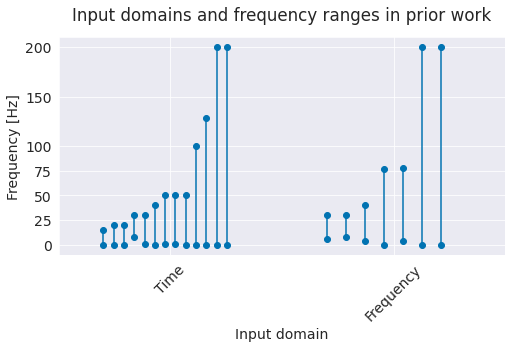
\includegraphics[width=1\linewidth]{latex_images/PriorWork_files/PriorWork_7_0.png}
    \caption[Input domains and frequency ranges in prior work.]{\textbf{Input domains and frequency ranges in prior work.} Grey linesrepresent frequency ranges of individual studies. Note that many studies
only include frequencies below 50 Hz, some use very restricted ranges
(alpha/beta band)}\label{input_domain_fig}
\end{figure}
    

    Deep networks can either decode directly from the time-domain EEG or
process the data in the frequency domain, for example after a Fourier
transformation. 12 of the prior studies used time-domain inputs, 6 used
frequency-domain inputs and one used both. We decided to work directly
in the time domain, as the deep networks should in principle be able to
learn how to extract any needed spectral information from the
time-domain input.

Most prior studies that were working in the time domain only used
frequencies below 50 Hz. We were interested in how well deep networks
can also extract higher-frequency components of the EEG
signal. For that, we used a sampling rate of 250 Hz, which means we were
able to analyze frequencies up to the Nyquist frequency of 125 Hz. As a
suitable dataset for high-frequency analysis, we
included our high-gamma dataset in our study, since it was recorded
specifically to allow extraction of higher-frequency (\textgreater50 Hz)
information from scalp EEG \citep{schirrmeisterdeephbm2017}.


\section{Network Architectures}\label{network-architectures}

    

\begin{figure}[th]
    \myfloatalign
    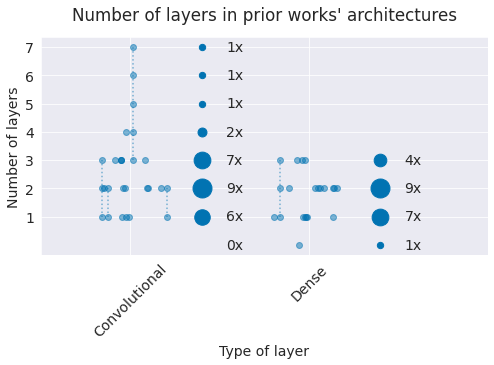
\includegraphics[width=0.9\linewidth]{latex_images/PriorWork_files/PriorWork_11_0.png}
    \caption[Number of layers in prior work.]{
\textbf{Number of layers in prior work.} Small grey markers represent
individual architectures. Dashed lines indicate different number of
layers investigated in a single study (e.g., a single study investigated
3-7 convolutional layers). Larger grey markers indicate sum of
occurences of that layer number over all studies (e.g., 9 architectures
used 2 convolutional layers). Note most architectures use only 1-3
convolutional layers.}\label{layernum_fig}
\end{figure}

    The architectures used in prior work typically only included up to 3
layers, with only 2 studies considering more layers. As network
architectures in other domains tend to be a lot deeper, we also
evaluated architectures with a larger number of layers in our work.
Several architectures from prior work also included fully-connected
layers with larger number of parameters which had fallen out of favor in
computer-vision deep-learning architectures due to their large compute
and memory requirements with little accuracy benefit. Our architectures
do not include traditional fully-connected layers with a large number of
parameters.



\section{Hyperparameter Evaluations}\label{hyperparameter-evaluations}

\begin{table}[ht]
    \small
    \myfloatalign
    \begin{tabularx}{\textwidth}{p{0.1\textwidth}p{0.4\textwidth}p{0.4\textwidth}} \toprule
        \tableheadlinewithwidth{0.1\textwidth}{\large Study} & \tableheadlinewithwidth{0.4\textwidth}{\large Design choices}
        & \tableheadlinewithwidth{0.4\textwidth}{\large Training strategies} \\ 
        \midrule
    \cite{lawhern_eegnet:_2016} & Kernel sizes & \\
\cite{sun_remembered_2016} & & Different time windows \\
\cite{tabar_novel_2017} & Addition of six-layer stacked
autoencoder on ConvNet features Kernel sizes & \\
\cite{liang_predicting_2016} & & Different subdivisions of
frequency range Different lengths of time crops Transfer learning with
auxiliary non-epilepsy datasets \\
\cite{hajinoroozi_eeg-based_2016} & Replacement of
convolutional layers by restricted Boltzmann machines with slightly
varied network architecture\} & \\
\cite{antoniades_deep_2016} & 1 or 2 convolutional layers
& \\
\cite{page_wearable_2016} & & Cross-subject supervised
training, within-subject finetuning of fully connected layers \\
\cite{bashivan_learning_2016} & Number of convolutional
layers Temporal processing of ConvNet output by max pooling, temporal
convolution, LSTM or temporal convolution + LSTM & \\
\cite{stober_learning_2016} & Kernel sizes & Pretraining
first layer as convolutional autoencoder with different constraints \\
\cite{sakhavi_parallel_2015} & Combination ConvNet and MLP
(trained on different features) vs.~only ConvNet vs.~only MLP & \\
\cite{stober_using_2014} & Best values from automatic
hyperparameter optimization: frequency cutoff, one vs two layers, kernel
sizes, number of channels, pooling width & Best values from automatic
hyperparameter optimization: learning rate, learning rate decay,
momentum, final momentum \\
\cite{wang_deep_2013} & Partially supervised CSA & \\
\cite{cecotti_convolutional_2011} & Electrode subset (fixed
or automatically determined) Using only one spatial filter Different
ensembling strategies & \\
        \bottomrule
    \end{tabularx}
    \caption[Design choices and training strategies of prior work.]{\textbf{Design choices and training strategies of prior work.}}  \label{prior-work-design-choices-table}
\end{table}

    Prior work varied widely in their comparison of design choices and
training strategies. 6 of the studies did not compare any design choices
or training strategy hyperparameters. The other 13 studies evaluated
different hyperparameters, with the most common one the kernel size (see
\Cref{prior-work-design-choices-table}). Only one study
evaluated a wider range of hyperparameters
\citep{stober_using_2014}. To fill this gap, we compared a
wider range of design choices and training strategies and specifically
evaluated whether improvements of computer vision architecture design
choices and training strategies also lead to improvements in EEG
decoding.


\section{Visualizations}\label{visualizations}

\begin{table}[ht]
    \small
    \myfloatalign
    \begin{tabularx}{\textwidth}{p{0.1\textwidth}p{0.2\textwidth}p{0.6\textwidth}} \toprule
        \tableheadlinewithwidth{0.1\textwidth}{\large Study} & \tableheadlinewithwidth{0.2\textwidth}{\large Type(s)}
        & \tableheadlinewithwidth{0.6\textwidth}{\large Findings} \\ 
        \midrule
\cite{sun_remembered_2016} & Weights (spatial) & Largest weights found over prefrontal and temporal cortex.\\
\cite{manor_multimodal_2016} & Weights, activations, gradient-based saliency maps & Weights showed typical P300 distribution. Activations were high at plausible times (300-500ms). Saliency maps showed plausible spatio-temporal plots.\\
\cite{tabar_novel_2017} & Weights (spatial + frequential) & Some weights represented difference of values of two electrodes on different sides of head.\\
\cite{liang_predicting_2016} & Weights,
clustering of weights & Clusters of weights showed typical frequency band subdivision (delta, theta, alpha, beta, gamma). \\
\cite{antoniades_deep_2016} & Weights, correlation weights and interictal epileptic discharges (IED), activations & Weights increasingly correlated with IED waveforms with increasing number of training iterations. Second layer captured more complex and well-defined epileptic shapes than first layer. IEDs led to highly synchronized activations for neighbouring electrodes. \\
\cite{thodoroff_learning_2016} & Input occlusion and effect on prediction accuracy & Allowed to locate areas critical for seizure. \\
\cite{george_single-trial_2016} & Weights (spatial) &  Some filter weights had expected topographic distributions for P300, others filters had large weights on areas not traditionally associated with P300.\\
\cite{bashivan_learning_2016} & Inputs that maximally activate given filter; Activations of these inputs, "Deconvolution" for these inputs & Different filters were sensitive to different frequency bands. Later layers had more spatially localized activations. Learned features had noticeable links to well-known electrophysiological markers of cognitive load.\\
\cite{stober_learning_2016} & Weights (spatial+3 timesteps, pretrained as autoencoder) & Different constraints led to different weights, one type of constraints could enforce weights that are similar across subjects. Other type of constraints led to weights that have similar spatial topographies under different architectural configurations and preprocessings. \\
\cite{manor_convolutional_2015} & Weights; Mean and single-trial activations & Spatiotemporal regularization led to softer peaks in weights. Spatial weights showed typical P300 distribution; Activations mostly had peaks at typical times (300-400ms). \\
\cite{cecotti_convolutional_2011} & Weights & Spatial filters were similar for different architectures. Spatial filters were different (more focal, more diffuse) for different subjects. \\
        \bottomrule
    \end{tabularx}
    \caption[Visualizations presented in prior work.]{\textbf{Visualizations presented in prior work.}}  \label{prior-work-visualizations-table}
\end{table}


    Visualizations can help understand what information the networks are
extracting from the EEG signal. 11 of the prior 19 studies presented any
visualizations. These studies mostly focused on analyzing weights and
activations, see \Cref{prior-work-visualizations-table}. In
our work, we first focused on investigating how far the networks extract
spectral features known to work well for movement-related decoding, see
\Cref{perturbation-visualization}. Later, we also developed
more sophisticated visualization methods and applied them both to
pathology decoding, see \Cref{invertible-networks} and
\Cref{understanding-pathology}.

\todotext{open question textbox}
